\documentclass[letterpaper, 12pt]{article}
\usepackage[utf8]{inputenc}
\usepackage[german]{babel} 
\usepackage[right=2.5cm,left=3cm,top=2cm,bottom=2cm]{geometry}
\usepackage{graphicx}
\usepackage{amsmath} 
\usepackage{amssymb}
\usepackage{mathrsfs}
\usepackage{latexsym}
\usepackage{dsfont}
\usepackage[usenames,dvipdsnames,svgnames,x11names]{xcolor}
\usepackage{enumerate}
\usepackage{enumitem}
\usepackage{array}
\usepackage{multirow}
\usepackage[style=apa]{biblatex}
\bibliography{bio}
\usepackage{fancyhdr}
\usepackage{hyperref}

\pagestyle{fancy}

    \fancyhf{}
    \chead{Problemas} 
    \lfoot{Villa Rosas Esteban}
    \rfoot{\thepage}


\begin{document}
\begin{center}

{\Huge{{\textbf{\emph{\underline{Problemas de Física Interesantes}}}}}}\\

{\small{Esteban Villa Rosas }}\\

{\small{November 04, 2022}}

\end{center}



\section{Problemas}

\begin{enumerate}

\item {{Considerando un sistema en una dimensión y sabiendo que $a=\frac{dv}{dt}$ y $v=\frac{dx}{dt}$ Demuestre que la posición se puede ver como:}}
    \begin{equation}
    \label{Ecuación de posición en el eje x}
        x=x_0 + v_0 t + \frac{1}{2} at^2
    \end{equation}
Para un tiempó inicial $t= 0 $ y con; $x_0$ y $v_0 $ la posición y la velocidad inicial en el sistema.\\\\
\underline{Dem}

Sabemos que 
\begin{equation}
    v=\frac{dx}{dt}
\end{equation}

\begin {equation}
\Longrightarrow\int_{0} ^{t} a = dt = \int_{v_0}^{v} dv
\end{equation}

\begin {equation}
\Longrightarrow at |_{0}^{t} = v |_{v_0}^{v} 
\end{equation}

\begin {equation}
\Longrightarrow at – a(0) = v – v_0
\end{equation}

\begin{equation}
\Longrightarrow at = v – v_0
\end{equation}

\begin{equation}
\label{Eq de velocidad}
\Longrightarrow v = v_0 + at 
\end{equation}

\begin{equation} 
\Longrightarrow v dt = dx 
\end{equation}
Sabemos que en la ecuación \ref{Eq de velocidad} nos da la velocidad, entonces sustituimos 
\begin{equation} 
(v_0 + at) dt = dx 
\end{equation}

\begin{equation} 
\Longrightarrow\int_{0} ^{t} (v_0 + at) dt =  _{x_0} ^{x} dx 
\end{equation}

\begin{equation}
\Longrightarrow v_0 t + \frac{at^2}{2} |_{0}^{t} = x |_{x_0}^{x}
\end{equation}

\begin{equation}
\Longrightarrow v_0 t + \frac{1}{2} at^2 = x – x_0
\end{equation}

\begin{equation}
\therefore x = x_0 + v_0 t + \frac{1}{2} at^2\textcolor{white}{iii} \blacksquare
\end{equation}
    
    \item Considere una carrera entre dos coches estos arrancan del reposo pero el coche uno hace trampa (cosa que nunca pasa), saliendo un segundo amtes que el segundo, si los autos tienen una aceleración de $3.5 m/s^2$  y  $4.9 m/s^2$ respectivamente.
    
\begin{enumerate}
    \item {¿En que momento el auto dos alcanza al auto uno i.e $t=?$}\\
Tenemos la formula que acabamos de demostrar \ref{Ecuación de posición en el eje x} por lo que podemos empezar a definir algunos datos que tenemos:\\\\
Auto 2: tiene una aceleración de $3.5m/s^2$
\begin{equation}
\label{Ecuacion inciso a auto 1}
    x= \frac{1}{2} a_{a1} t^2 
\end{equation}
\begin{equation}
\label{Ecuación inciso a auto 2}
     x= \frac{1}{2} (3.5 m/s^2)(t-1s)^2 
\end{equation}
\\
Auto 1: tiene una aceleración de $4.9m/s^2$
\\
\begin{equation}
    x = \frac{1}{2} a_{a2}t^2
\end{equation}
\begin{equation}
    x = \frac{1}{2} (4.9 m/s^2)t^2
\end{equation}
\\
Igualamos las dos ecuaciones que nos dieron y desarrollamos hasta encontrar $t$.
\begin{equation}
\label{Eq inciso 2 ya igualada}
    \frac{1}{2} (3.5 m/s^2)(t-1s)^2 = \frac{1}{2} (4.9 m/s^2)t^2
\end{equation}

\begin{equation}
    \frac{3.5}{2} (t^2 - 2t + 1) = \frac{4.9}{2} t^2
\end{equation}
\begin{equation}
    \frac{3.5t^2 - 7t + 3.5}{2} = \frac{4.9}{2} t^2
\end{equation}
\begin{equation}
    (2)(\frac{3.5t^2 - 7t + 3.5}{2}) = 4.9t^2
\end{equation}
\begin{equation}
    3.5t^2 - 7t + 3.5 = 4.9t^2
\end{equation}
Igualamos a 0:
\begin{equation}
    3.5t^2 - 7t + 3.5 - 4.9t^2 = 0
\end{equation}
\begin{equation}
    -1.4t^2 - 7t + 3.5  = 0
\end{equation}

\begin{equation}
    -\frac{7}{5}t^2 - 7t + \frac{7}{2}  = 0
\end{equation}
\begin{equation}
    2t^2 + 10t -5 = 0
\end{equation}
Una vez igualada a 0 podemos resolverla por la formula general la cual es 
\begin{equation}
     x = \frac{-b \pm \sqrt{b^2 - 4ac}}{2a}
\end{equation}

\begin{equation}
    t = \frac{- 10 \pm \sqrt{-10^2 - 4(2)(-5)}}{2(2)}
\end{equation}
\begin{equation}
    t = \frac{- 10 \pm \sqrt{100+40}}{4}
\end{equation}
\begin{equation}
    t = \frac{- 10 \pm \sqrt{140}}{4}
\end{equation}

\begin{equation}
    t_1 = \frac{- 10 - \sqrt{140}}{4}
\end{equation}
\begin{equation}
\label{Ecuacion t_1 del inciso a}
    t_1 = -5.45804
\end{equation}

\begin{equation}
    t_2 = \frac{- 10 + \sqrt{140}}{4}
\end{equation}
\begin{equation}
    t_2 = 0.4504
\end{equation}

El tiempo en que el auto tarda en alcanzarlo es de $5.45$ segundos .

    \item ¿Cuál será la posición cuando el inciso (a) ocurra $x=?$\\
Debemos sustituir los valores que ya tenemos en la ecuación \ref{Ecuación de posición en el eje x}.
    \begin{equation}
    x=x_0 + v_0 t + \frac{1}{2} at^2
    \end{equation}
Sustituimos:
    \begin{equation}
    x= \frac{1}{2} (3.5m/s^2)(5.45+1)^2
    \end{equation}
Nos queda:
\begin{equation}
    72.9859m
\end{equation}
Ahora sustituimos en la ecuación \ref{Ecuación inciso a auto 2}.

    \begin{equation}
    x= \frac{1}{2} (4.9m/s^2)(5.45)^2
    \end{equation}
Nos queda:
\begin{equation}
    72.9859m
\end{equation}
Por lo tanto $x=72.9859m$
    \item ¿Cuál será la velocidad que tendrá en ese punto para ambos autos?
    
La Velocidad con aceleración de 4.90$m/s^2$es:
\begin{equation}
    v = a_1 t
\end{equation}
\begin{equation}
    v = (4.90m/s^2)(5.45s)
\end{equation}
\begin{equation}
    v = 26.8 m/s
\end{equation}
Por otro lado, la velocidad en el auto con la aceleración de 3.5$m/s^2$es:
\begin{equation}
\label{Ecuación v}
    v = a_2 t
\end{equation}
\begin{equation}
    v = (3.5m/s^2)(6.45s)
\end{equation}
\begin{equation}
    v = 22.6 m/s
\end{equation}


    \item Toma 5 tiempos diferentes a partir de que los autos arrancan, sin tomar el tiempo inicial, 3 antes del tiempo donde los autos se encuentran y dos posteriores a ese tiempo, realicen dos tablas, una para cada auto, con la siguiente información; aceleración, tiempo posición y velocidad.\\


 \begin{table}[h]
\label{Tabla de 3.5)}
    \centering
\caption{{Cinemática del Auto con Aceleración 3.5$m/s^2$}}

\begin{tabular}{c|c|c|c|c|c} \hline \hline
\multicolumn{6}{c}{Auto con Aceleración 3.5$m/s^2$}\\\hline 
\multicolumn{3}{c|}{No dependiente del tiempo} & \multicolumn{3}{c}{Dependientes del tiempo}\\\hline
\multicolumn{3}{c|} {$a[m/s^2]$} & $t[s]$ & $x[m]$ & $v[m/s]$  \\ \hline
\multicolumn{3}{c|}{} &2s  &7m &7m/s \\\cline{4-6}
\multicolumn{3}{c|}{} &3s  &15.75m &10.5m/s \\ \cline{4-6}
\multicolumn{3}{c|} {3.5$m/s^2$} &4s &28m &14m/s  \\ \cline{4-6}
\multicolumn{3}{c|}{} &6s  &63m &21m/s \\ \cline{4-6}
\multicolumn{3}{c|}{} &7s  &85.75m &24.5m/s\\ \hline \hline
\end{tabular}\\
  \end{table}
 
\vspace{2cm} 
Para obtener los valores de la tabla \ref{Tabla de 3.5)}
debemos sustituir los tiempos en las ecuaciones:\\\\
Para la distancia:
    \begin{equation}
    x= \frac{1}{2} at^2
    \end{equation} 
Para la velocidad:
\begin{equation}
    v = at
\end{equation}
\end{enumerate}
\\
\vspace{1cm}

 \begin{table}[h]
\label{Tabla de auto 4.9}
    \centering
\caption{{Cinemática del Auto con aceleración 4.9$m/s^2$}}

\begin{tabular}{c|c|c|c|c|c} \hline \hline
\multicolumn{6}{c}{Auto con aceleración 4.9$m/s^2$}\\\hline 
\multicolumn{3}{c|}{No dependiente del tiempo} & \multicolumn{3}{c}{Dependientes del tiempo}\\\hline
\multicolumn{3}{c|} {$a[m/s^2]$} & $t[s]$ & $x[m]$ & $v[m/s]$  \\ \hline
\multicolumn{3}{c|}{} &2s &9.8m &9.8m/s  \\\cline{4-6}
\multicolumn{3}{c|}{} &3s &22.05m &14.7m/s \\ \cline{4-6}
\multicolumn{3}{c|} {4.9$m/s$} &4s &39.2m &19.6m/s   \\ \cline{4-6}
\multicolumn{3}{c|}{} &6s &88.2m  &29.4m/s  \\ \cline{4-6}
\multicolumn{3}{c|}{} &7s &120.05m  &34.3m/s \\ \hline \hline
\end{tabular}\\
  \end{table}


Para obtener los valores de la tabla \ref{Tabla de auto 4.9} debemos sustituir los tiempos en las ecuaciones:\\\\
   Para la distancia:
    \begin{equation}
    x= \frac{1}{2} at^2
    \end{equation} 
Para la velocidad:
\begin{equation}
    v = at
\end{equation}

\newpage
    \item Considere el siguiente sistema, dos bloques de masas $m1$ y $m2$ estan unidos por una cuerda ideal y descansan sobre una superficie horizontal sin roce. Si una fuerza de magintud $A$ se le aplica al bloque de masa $m2$ horizontalmente, en la dirección que muestra la Figura 1. Realicen los respectivos diagramas de cuerpos libres (usen powerpoint, pait, dibújelo, lo que gusten) y anexelo   como una imagen, a partir de ellos determinen la aceleración del sistema y la tensión de la cuerda entre los bloques.\\

En la imagen se presenta el diagrama de cuerpo libre donde se reprentan de manera grafica las fuerzas que estan sobre los cuerpos de masa $m_1$ y $m_2$. La formula de la segunda ley de Newton es:
\begin{equation}
\label{Eq Segunda ley}
    F = ma
\end{equation}
Observe que tenemos dos masas por lo que en la ecuación \ref{Eq Segunda ley}
vamos a sustituir la m por la suma de las dos masas
\begin{equation}
    F = (m_1 + m_2)a
\end{equation}
Entonces la tensión $t - t$ seria $m_1 a$.
Por lo tanto:
\begin{equation}
    T = (m_1 -m_2)a + A
\end{equation}

\end{enumerate}
    \begin{figure}
    \centering
        \caption{Diagrama de cuerpo libre }
    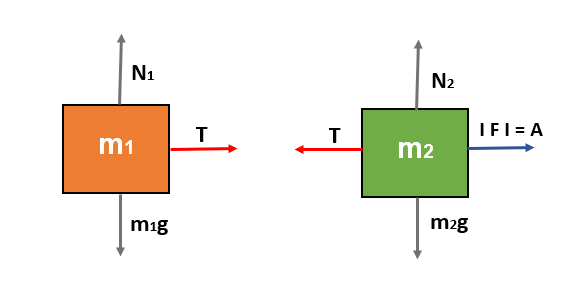
\includegraphics[scale=0.70]{Diagrama de cuerpo libre.png}

    \label{fig, diagrama}
\end{figure}

\pagestyle{fancy}

    \fancyhf{}
    \chead{Punto Extra} 
    \lfoot{Villa Rosas Esteban}
    \rfoot{\thepage}
    
\section{Punto Extra}
\begin{itemize}
    \item Investiguen que hace la paqueteria ``hyperref'' y expliquen que hace, citen su fuente
    donde fue investigado.\\
    
Hacer un documento navegable es tan sencillo como cargar el paquete ``hyperref'', automáticamente las referencias en el texto y la tabla de contenidos se convierten en ``links'' que nos llevan hasta la referencia o la sección correspondiente. Puesto que el paquete
hyperref redefine muchos comandos LATEX es conveniente que sea el último paquete
en cargarse.
Para cargarlo, se utiliza la sintaxis habitual:
usepackage[opciones]{hyperref}\\
Este comando se utiliza para poder hacer referencias de una manera mas creativa, por ejemplo, en este documento al tocar el número encerrado con color rojo nos va a dirigir a la ecuación, tabla o imagen a la que se está citando dentro del documento para así no volver a escribir cada escuación de nuevo.
\end{itemize}

\begin{thebibliography}{}
\bibitem{}. (2022). Retrieved 6 November 2022, from https://mat.uda.cl/hsalinas/cursos/2008/latex/apuntes10.pdf

\end{thebibliography}

\end{document}